\chapter{Examples of Some Special Cases}\label{chap:examples}

Lorem ipsum dolor sit amet, consectetur adipiscing elit. Aliquam ac malesuada leo. Aliquam sit amet eros eleifend, molestie quam eu, scelerisque tortor. Etiam vel diam rutrum, maximus arcu nec, tempus magna. Praesent pretium, mauris eget euismod facilisis, libero lorem laoreet leo, at bibendum arcu massa at dui. Aliquam id felis mi. Vivamus egestas efficitur metus, sed semper libero facilisis in. Cras id scelerisque quam, sit amet dictum tellus. Integer porttitor laoreet iaculis. In hac habitasse platea dictumst. Nullam justo ante, lacinia in tristique sed, vehicula in purus. Phasellus condimentum dapibus mauris, id molestie tortor. Nullam vel ante nulla. Etiam aliquam varius sem, sit amet luctus massa rhoncus in. Praesent eget ex nec lacus tincidunt facilisis nec id ligula. Quisque sollicitudin, massa vitae laoreet aliquam, tortor lacus condimentum ligula, vitae sodales velit mauris ut magna. Duis eleifend vulputate ultricies.

\begin{figure}[htbp]
    \centering
    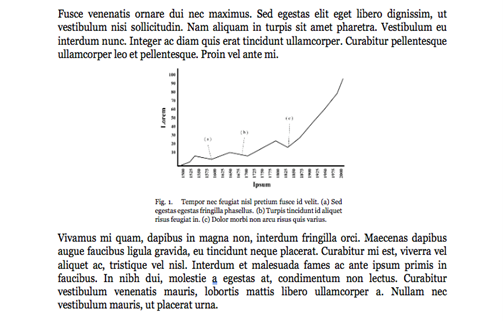
\includegraphics[width=\linewidth]{Figures/Picture1.png}
    \caption{Figure Interrupting The Paragraphs}
    \label{fig:e1}
\end{figure}

\red{This is one of the special cases, we have included the Fig.~\ref{fig:e1} before this paragraph in the code editor. However, the space in the rest of the page is not enough. In this case, the figure will be arranged the first available place in the next page, even interrupting the paragraph afterwards. To solve this, the best way is to manually change the place where the figure is included in the code editor.}

Lorem ipsum dolor sit amet, consectetur adipiscing elit. Aliquam ac malesuada leo. Aliquam sit amet eros eleifend, molestie quam eu, scelerisque tortor. Etiam vel diam rutrum, maximus arcu nec, tempus magna. Praesent pretium, mauris eget euismod facilisis, libero lorem laoreet leo, at bibendum arcu massa at dui. Aliquam id felis mi. Vivamus egestas efficitur metus, sed semper libero facilisis in. Cras id scelerisque quam, sit amet dictum tellus. Integer porttitor laoreet iaculis. In hac habitasse platea dictumst. Nullam justo ante, lacinia in tristique sed, vehicula in purus. Phasellus condimentum dapibus mauris, id molestie tortor. Nullam vel ante nulla. Etiam aliquam varius sem, sit amet luctus massa rhoncus in. Praesent eget ex nec lacus tincidunt facilisis nec id ligula. Quisque sollicitudin, massa vitae laoreet aliquam, tortor lacus condimentum ligula, vitae sodales velit mauris ut magna. Duis eleifend vulputate ultricies. \red{Here we break into a new page to show the same case and how to handle it.}

\newpage

Lorem ipsum dolor sit amet, consectetur adipiscing elit. Aliquam ac malesuada leo. Aliquam sit amet eros eleifend, molestie quam eu, scelerisque tortor. Etiam vel diam rutrum, maximus arcu nec, tempus magna. Praesent pretium, mauris eget euismod facilisis, libero lorem laoreet leo, at bibendum arcu massa at dui. Aliquam id felis mi. Vivamus egestas efficitur metus, sed semper libero facilisis in. Cras id scelerisque quam, sit amet dictum tellus. Integer porttitor laoreet iaculis. In hac habitasse platea dictumst. Nullam justo ante, lacinia in tristique sed, vehicula in purus. Phasellus condimentum dapibus mauris, id molestie tortor. Nullam vel ante nulla. Etiam aliquam varius sem, sit amet luctus massa rhoncus in. Praesent eget ex nec lacus tincidunt facilisis nec id ligula. Quisque sollicitudin, massa vitae laoreet aliquam, tortor lacus condimentum ligula, vitae sodales velit mauris ut magna. Duis eleifend vulputate ultricies. Nullam vel ante nulla. Etiam aliquam varius sem, sit amet luctus massa rhoncus in. Praesent eget ex nec lacus tincidunt facilisis nec id ligula. Quisque sollicitudin, massa vitae laoreet aliquam, tortor lacus condimentum ligula, vitae sodales velit mauris ut magna. Duis eleifend vulputate ultricies.

\blue{This is the example of how to handle this manually. This is the place where Fig.~\ref{fig:e2} is first time referred to. The space in the rest of the page is not enough. We have changed the place where the figure is included. Please check the code editor to see the changes.}

Lorem ipsum dolor sit amet, consectetur adipiscing elit. Aliquam ac malesuada leo. Aliquam sit amet eros eleifend, molestie quam eu, scelerisque tortor. Etiam vel diam rutrum, maximus arcu nec, tempus magna. Praesent pretium, mauris eget euismod facilisis, libero lorem laoreet leo, at bibendum arcu massa at dui. Aliquam id felis mi. Vivamus egestas efficitur metus, sed semper libero facilisis in. Cras id scelerisque quam, sit amet dictum tellus. Integer porttitor laoreet iaculis. In hac habitasse platea dictumst. Nullam justo ante, lacinia in tristique sed, vehicula in purus. Phasellus condimentum dapibus mauris, id molestie tortor. Nullam vel ante nulla. Etiam aliquam varius sem, sit amet luctus massa rhoncus in. Praesent eget ex nec lacus tincidunt facilisis nec id ligula.  \blue{We includ the Fig.~\ref{fig:e2} after this paragraph in the code editor. In this way, there is enough space for the figure between the paragraphs. Including tables should also be in the same way.}

\begin{figure}[htbp]
    \centering
    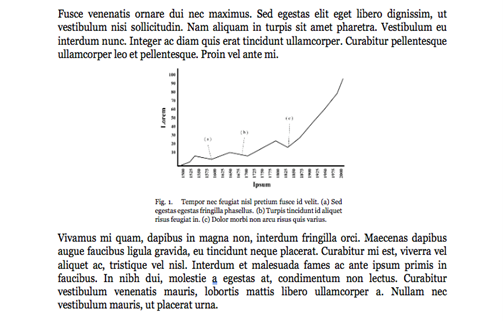
\includegraphics[width=\linewidth]{Figures/Picture1.png}
    \caption{Figure Not Interrupting The Paragraphs}
    \label{fig:e2}
\end{figure}

Lorem ipsum dolor sit amet, consectetur adipiscing elit. Aliquam ac malesuada leo. Aliquam sit amet eros eleifend, molestie quam eu, scelerisque tortor. 

\newpage

Lorem ipsum dolor sit amet, consectetur adipiscing elit. Aliquam ac malesuada leo. Aliquam sit amet eros eleifend, molestie quam eu, scelerisque tortor. Etiam vel Quisque sollicitudin, massa vitae laoreet aliquam, tortor lacus condimentum ligula, vitae sodales velit mauris vitae sodales vut mauris magna. \red{Another special case is, when writing some formula or some explanations, you may write in this way: Lorem ipsum dolor sit amet, consectetur adipiscing adipis  elit. here we denote the second as $s$.}

\blue{You will find that the character $s$ is isolated at the beginning of a new line. This should be avoid. The way to solve this is also included in the very beginning of Dissertation.tex. You can find the solution using \textasciitilde~ in the code editor in the next paragraph.}

Lorem ipsum dolor sit amet, consectetur adipiscing elit. Aliquam ac malesuada leo. Aliquam sit amet eros eleifend, molestie quam eu, scelerisque tortor. Etiam vel Quisque sollicitudin, massa vitae laoreet aliquam, tortor lacus condimentum ligula, vitae sodales velit mauris vitae sodales vut mauris magna. \red{Another special case is, when writing some formula or some explanations, you may write in this way: Lorem ipsum dolor sit amet, consectetur adipiscing adipis  elit. here we denote the second as~$s$.} 

\blue{In this way writing as ``as\textasciitilde$s$'' in the code editor, ``as~$s$'' will be considered to be rendered together to avoid the isolated character in a new line.} It is also recommended always connect your references or refers with a \textasciitilde. Read the code editor for details, e.g. Lorem ipsum~\cite{EI-CPS-Book}, Lorem ipsum Fig.~\ref{fig:e2}.